\documentclass[12pt]{article}

\usepackage{sbc-template}
\usepackage{graphicx,url}
\usepackage[utf8]{inputenc}
\usepackage[T1]{fontenc}
\usepackage[brazil]{babel}
\usepackage{amsmath}
\usepackage{booktabs}
\usepackage{float}

\title{Detecção de Contas Fraudulentas na Rede Ethereum:\\ Uma Abordagem Comparativa de Algoritmos de Classificação}

\author{Mateus Medeiros Schneider\inst{1}}

\address{Instituto Federal de Educação, Ciência e Tecnologia do Rio Grande do Sul --
Campus Ibirubá\\
  Rua Nelsi Ribas Fritsch, 1111 -- CEP: 98200-000 -- Ibirubá -- RS -- Brasil
  \email{2023009762@aluno.ibiruba.ifrs.edu.br}
}

\begin{document}

\renewcommand{\tablename}{Tabela}
\renewcommand{\figurename}{Figura}

\maketitle

\begin{abstract}
This paper presents a data mining process, following the CRISP-DM
methodology, for detecting fraudulent accounts on the Ethereum
blockchain. Using a public dataset of 9,841 accounts described by
aggregated transaction attributes, six classification algorithms were
compared through stratified cross-validation. After hyperparameter
optimization, Random Forest achieved the best performance, with an
F1-score of 0.9832 and AUC-ROC of 0.9993 on the test set, with zero
false positives. The interpretation of the most relevant attributes
revealed behavioral patterns characteristic of fraudulent accounts,
such as low transaction counts and absence of ERC20 token activity.
\end{abstract}

\begin{resumo}
Este trabalho apresenta um processo de mineração de dados, seguindo a
metodologia CRISP-DM, para a detecção de contas fraudulentas na rede
\textit{blockchain} Ethereum. Utilizando um conjunto de dados público
com 9.841 contas descritas por atributos agregados de transações, foram
comparados seis algoritmos de classificação por meio de validação
cruzada estratificada. Após a otimização de hiperparâmetros, o algoritmo
Random Forest obteve o melhor desempenho, com F1-score de 0,9832 e
AUC-ROC de 0,9993 no conjunto de teste, sem nenhum falso positivo. A
interpretação dos atributos mais relevantes revelou padrões
comportamentais característicos de contas fraudulentas, como baixo
número de transações e ausência de atividade com tokens ERC20.
\end{resumo}

\section{Introdução}

A popularização das criptomoedas trouxe, junto com a promessa de
transações descentralizadas e sem intermediários, um aumento expressivo
de golpes financeiros. A rede Ethereum, por permitir a execução de
contratos inteligentes e a criação de tokens, tornou-se um ambiente
atrativo tanto para aplicações legítimas quanto para esquemas
fraudulentos, como golpes de \textit{phishing}, esquemas Ponzi e
contas usadas exclusivamente para lavagem de valores.

Diferentemente do sistema bancário tradicional, no qual há instituições
centralizadas responsáveis por monitorar transações suspeitas, na
\textit{blockchain} a responsabilidade pela identificação de fraudes
recai sobre as próprias plataformas que intermediam o acesso dos
usuários, como corretoras (\textit{exchanges}) e carteiras digitais.
Nesse contexto, a detecção automática de contas com comportamento
fraudulento a partir do histórico de transações é uma ferramenta
relevante para a proteção dos usuários.

O \textbf{objetivo de negócio} deste trabalho é permitir que
\textit{exchanges}, provedores de carteiras digitais e plataformas
descentralizadas identifiquem preventivamente contas com comportamento
potencialmente fraudulento na rede Ethereum, reduzindo perdas
financeiras de usuários e fortalecendo a segurança do ecossistema. O
\textbf{objetivo de mineração de dados}, por sua vez, é desenvolver e
comparar modelos de classificação binária capazes de prever se uma
conta Ethereum é fraudulenta ou legítima a partir de atributos
agregados de seu histórico de transações, avaliando diferentes
algoritmos por meio de métricas como precisão, \textit{recall},
F1-score e AUC.

O restante deste artigo está organizado da seguinte forma: a Seção 2
apresenta o referencial teórico e os trabalhos correlatos; a Seção 3
detalha a metodologia, contemplando a compreensão dos dados, a
preparação e a modelagem; a Seção 4 apresenta e discute os resultados;
e a Seção 5 conclui o trabalho e aponta direções futuras.

\section{Referencial Teórico e Trabalhos Correlatos}

\subsection{Mineração de Dados e o Processo CRISP-DM}

A mineração de dados consiste na aplicação de algoritmos para a
extração de conhecimento implícito e útil a partir de grandes volumes
de dados \cite{fayyad1996}. Para conduzir esse processo de forma
estruturada, este trabalho adota a metodologia CRISP-DM
(\textit{Cross-Industry Standard Process for Data Mining}), composta
pelas etapas de compreensão do negócio, compreensão dos dados,
preparação dos dados, modelagem, avaliação e implantação.

\subsection{Classificação Supervisionada}

A tarefa de classificação consiste em aprender uma função que mapeie um
conjunto de atributos a um rótulo de classe pré-determinado
\cite{tan2009}. Neste trabalho são avaliados seis algoritmos
amplamente utilizados: Regressão Logística, Árvore de Decisão, Random
Forest, \textit{Naive Bayes}, K-vizinhos mais próximos (KNN) e Máquina
de Vetores de Suporte (SVM). O Random Forest é um método de
\textit{ensemble} que combina múltiplas árvores de decisão treinadas
sobre subconjuntos aleatórios dos dados, reduzindo o sobreajuste e
aumentando a robustez das previsões.

\subsection{Detecção de Fraude em \textit{Blockchain}}

A detecção de fraude em redes \textit{blockchain} tem sido abordada na
literatura por meio de técnicas de aprendizado de máquina aplicadas a
atributos extraídos do histórico de transações das contas. Esses
atributos incluem volume e frequência de transações, valores médios
movimentados e interações com diferentes tipos de tokens. A principal
dificuldade nesse domínio é o forte desbalanceamento entre classes,
uma vez que contas fraudulentas representam uma minoria do total de
contas observadas, exigindo estratégias específicas de tratamento.

\section{Metodologia}

Este trabalho adota uma abordagem quantitativa experimental, seguindo
as etapas do CRISP-DM. O desenvolvimento foi realizado em linguagem
Python, com as bibliotecas \textit{pandas} e \textit{numpy} para
manipulação de dados e \textit{scikit-learn} para a implementação dos
algoritmos de classificação, validação cruzada e otimização de
hiperparâmetros. As visualizações foram geradas com \textit{matplotlib}.

\subsection{Compreensão dos Dados}

O conjunto de dados utilizado é o \textit{Ethereum Fraud Detection
Dataset}, disponível publicamente na plataforma Kaggle\footnote{Disponível
em: \url{https://www.kaggle.com/datasets/vagifa/ethereum-frauddetection-dataset}}.
O \textit{dataset} contém 9.841 contas da rede Ethereum, descritas por
50 atributos, além da variável alvo \textit{FLAG}, que indica se a
conta é fraudulenta (1) ou legítima (0).

Os atributos descrevem o comportamento transacional agregado de cada
conta, incluindo o número de transações enviadas e recebidas, o tempo
médio entre transações, os valores mínimo, máximo e médio de Ether
movimentado, o número de endereços únicos com os quais a conta
interagiu e estatísticas relativas a transações de tokens ERC20.

A análise exploratória revelou um forte desbalanceamento entre as
classes: das 9.841 contas, 7.662 (77,86\%) são legítimas e apenas 2.179
(22,14\%) são fraudulentas, conforme ilustrado na Figura
\ref{fig:dist}. Esse desbalanceamento foi um fator determinante na
escolha das métricas de avaliação e nas estratégias de tratamento
adotadas.

\begin{figure}[H]
\centering
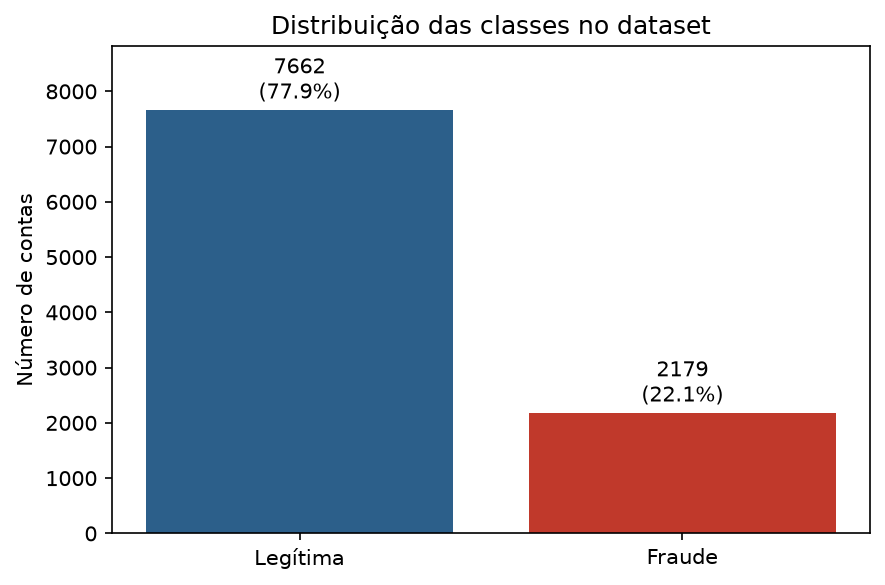
\includegraphics[width=0.6\textwidth]{fig1_class_distribution.png}
\caption{Distribuição das classes no conjunto de dados.}
\label{fig:dist}
\end{figure}

Foram também identificados outros problemas de qualidade nos dados:
(i) 25 das 51 colunas apresentavam valores ausentes, concentrados nos
atributos de tokens ERC20, indicando contas sem qualquer atividade
desse tipo; (ii) sete colunas relativas a tempos entre transações de
contrato ERC20 possuíam variância zero (valor constante); (iii) uma
coluna estava duplicada por erro no cabeçalho original do arquivo; e
(iv) cerca de 9,9\% das contas apresentavam saldo total de Ether
negativo, uma inconsistência física que, no entanto, mostrou-se
associada de forma sistemática à classe da conta, sendo, portanto,
preservada.

\subsection{Preparação dos Dados}

A etapa de preparação seguiu um conjunto de decisões documentadas,
implementadas em um \textit{pipeline} reproduzível:

\begin{itemize}
\item \textbf{Remoção de colunas}: foram eliminados os identificadores
(índice e endereço da conta), as sete colunas de variância zero e a
coluna duplicada, por não agregarem valor preditivo.

\item \textbf{Tratamento de valores ausentes}: identificaram-se três
representações distintas para ``ausência de atividade ERC20'' (valor
nulo, \textit{string} ``0'' e \textit{string} vazia), que foram
unificadas em uma única categoria \textit{None}. Os atributos
numéricos ERC20 ausentes foram preenchidos com zero, pois a ausência,
nesses casos, representa a inexistência de transações.

\item \textbf{Redução de cardinalidade}: as colunas categóricas de tipo
de token, que possuíam 304 e 466 categorias distintas, foram reduzidas
aos dez tokens mais frequentes, agrupando os demais em uma categoria
\textit{Other}.

\item \textbf{Transformação logarítmica}: os atributos monetários e de
contagem apresentavam forte assimetria (com coeficientes de até 62).
Aplicou-se uma transformação logarítmica assinada,
$\text{sign}(x)\cdot\log(1+|x|)$, que reduziu a assimetria para valores
entre 0,6 e 1,5, preservando o sinal de atributos que podem ser
negativos, como o saldo total.

\item \textbf{Codificação e divisão}: as variáveis categóricas foram
codificadas via \textit{one-hot encoding}. Os dados foram divididos em
75\% para treino e 25\% para teste, de forma estratificada, preservando
a proporção entre classes. Por fim, os atributos foram padronizados com
\textit{StandardScaler}, ajustado exclusivamente no conjunto de treino
para evitar vazamento de dados.
\end{itemize}

Após o pré-processamento, o conjunto final ficou com 61 atributos e
nenhum valor ausente.

\subsection{Modelagem}

A modelagem foi conduzida em duas etapas. Primeiro, os seis algoritmos
candidatos foram comparados por meio de validação cruzada estratificada
de 5 dobras (\textit{5-fold}) sobre o conjunto de treino, utilizando o
F1-score como métrica principal -- mais informativa que a acurácia em
cenários desbalanceados. Os algoritmos que admitem tratamento de
classes desbalanceadas foram configurados com o parâmetro
\textit{class\_weight} ajustado para ``balanced''.

Em seguida, os dois modelos mais relevantes foram submetidos à
otimização de hiperparâmetros via \textit{GridSearchCV}: o Random
Forest, por apresentar o melhor desempenho bruto, e a Regressão
Logística, por oferecer interpretabilidade direta por meio de seus
coeficientes. A estratégia de validação na otimização também foi a
validação cruzada estratificada de 5 dobras.

\section{Resultados e Discussão}

\subsection{Comparação entre Algoritmos}

A Figura \ref{fig:comp} apresenta o F1-score médio obtido por cada
algoritmo na validação cruzada. Observa-se que cinco dos seis
algoritmos alcançaram desempenho elevado (F1 superior a 0,94), com
destaque para o Random Forest (F1 = 0,9778). O algoritmo \textit{Naive
Bayes}, por outro lado, apresentou desempenho substancialmente inferior
(F1 = 0,5139).

\begin{figure}[H]
\centering
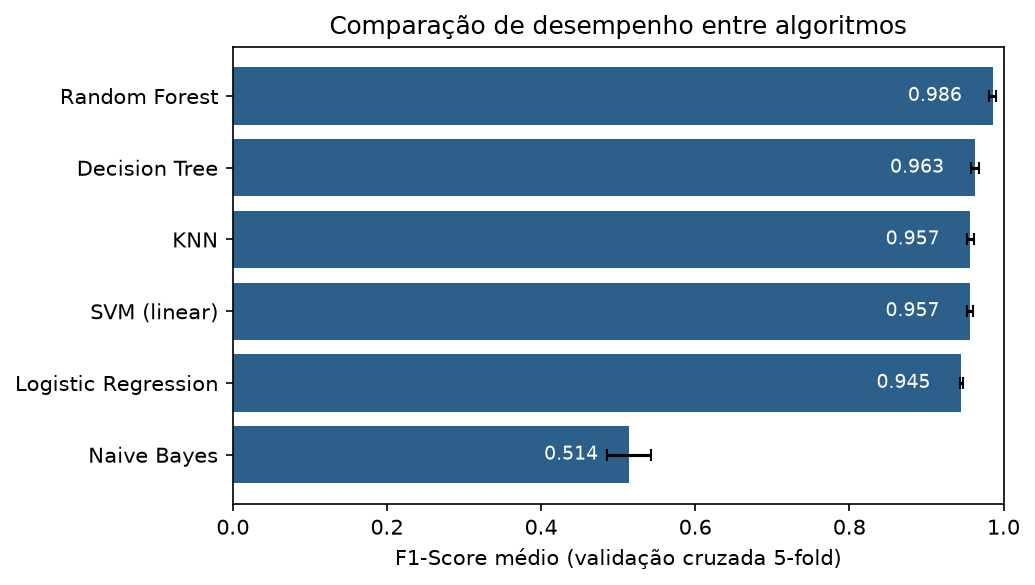
\includegraphics[width=0.75\textwidth]{fig2_model_comparison.png}
\caption{Comparação do F1-score médio entre os algoritmos
(validação cruzada de 5 dobras).}
\label{fig:comp}
\end{figure}

O baixo desempenho do \textit{Naive Bayes} é explicado por sua
suposição de independência condicional e de distribuição normal dos
atributos, premissas que não se sustentam neste conjunto de dados, no
qual coexistem atributos contínuos fortemente correlacionados e
atributos binários resultantes da codificação \textit{one-hot}. Esse
resultado reforça observações da literatura sobre as limitações desse
algoritmo em cenários com atributos correlacionados.

A Tabela \ref{tab:cv} apresenta as métricas detalhadas da validação
cruzada para todos os algoritmos.

\begin{table}[H]
\centering
\caption{Métricas médias na validação cruzada (5-fold).}
\label{tab:cv}
\begin{tabular}{lccccc}
\toprule
\textbf{Modelo} & \textbf{F1} & \textbf{AUC-ROC} & \textbf{Precisão} & \textbf{Recall} & \textbf{Acurácia} \\
\midrule
Random Forest        & 0,9778 & 0,9993 & 1,0000 & 0,9565 & 0,9904 \\
Árvore de Decisão    & 0,9619 & 0,9743 & 0,9655 & 0,9584 & 0,9832 \\
KNN                  & 0,9572 & 0,9881 & 0,9798 & 0,9357 & 0,9814 \\
SVM (linear)         & 0,9569 & 0,9911 & 0,9358 & 0,9792 & 0,9805 \\
Regressão Logística  & 0,9452 & 0,9943 & 0,9202 & 0,9718 & 0,9751 \\
\textit{Naive Bayes} & 0,5139 & 0,8970 & 0,3507 & 0,9657 & 0,5927 \\
\bottomrule
\end{tabular}
\end{table}

\subsection{Avaliação dos Modelos Otimizados}

Após a otimização, os dois modelos selecionados foram avaliados no
conjunto de teste, não utilizado em nenhuma etapa anterior. A Tabela
\ref{tab:final} resume os resultados, e a Figura \ref{fig:cm} apresenta
as matrizes de confusão.

\begin{table}[H]
\centering
\caption{Resultados finais no conjunto de teste.}
\label{tab:final}
\begin{tabular}{lccc}
\toprule
\textbf{Modelo} & \textbf{F1-Score} & \textbf{AUC-ROC} & \textbf{AUC-PR} \\
\midrule
Random Forest (otimizado)       & 0,9832 & 0,9993 & 0,9979 \\
Regressão Logística (otimizada) & 0,9597 & 0,9950 & 0,9885 \\
\bottomrule
\end{tabular}
\end{table}

\begin{figure}[H]
\centering
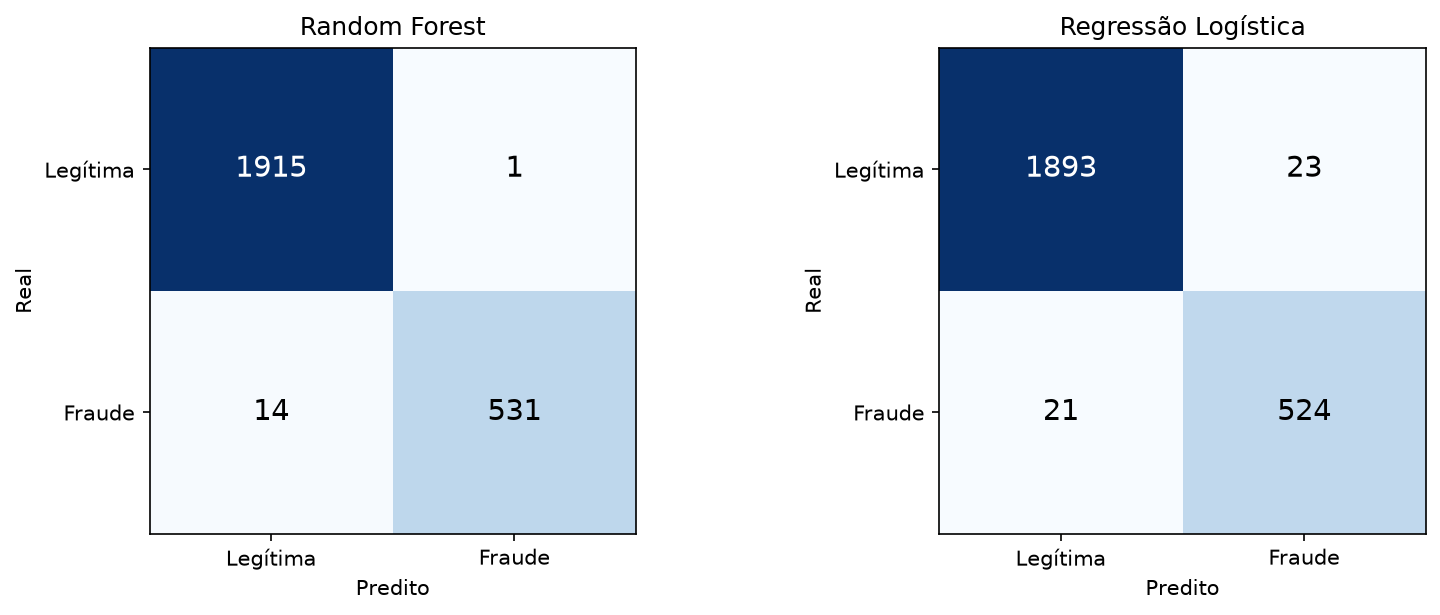
\includegraphics[width=0.9\textwidth]{fig3_confusion_matrices.png}
\caption{Matrizes de confusão dos modelos otimizados no conjunto
de teste.}
\label{fig:cm}
\end{figure}

O Random Forest obteve o melhor desempenho, com F1-score de 0,9832 e,
notavelmente, nenhum falso positivo -- ou seja, nenhuma conta legítima
foi incorretamente classificada como fraudulenta. Esse resultado é
particularmente relevante para o objetivo de negócio, pois o bloqueio
indevido de uma conta legítima representa um custo elevado em termos de
experiência do usuário e reputação da plataforma. O modelo deixou de
identificar apenas 18 das 545 contas fraudulentas do conjunto de teste.

As curvas ROC e Precision-Recall, apresentadas na Figura
\ref{fig:curves}, confirmam a superioridade do Random Forest, que
mantém precisão elevada ao longo de praticamente toda a faixa de
\textit{recall}.

\begin{figure}[H]
\centering
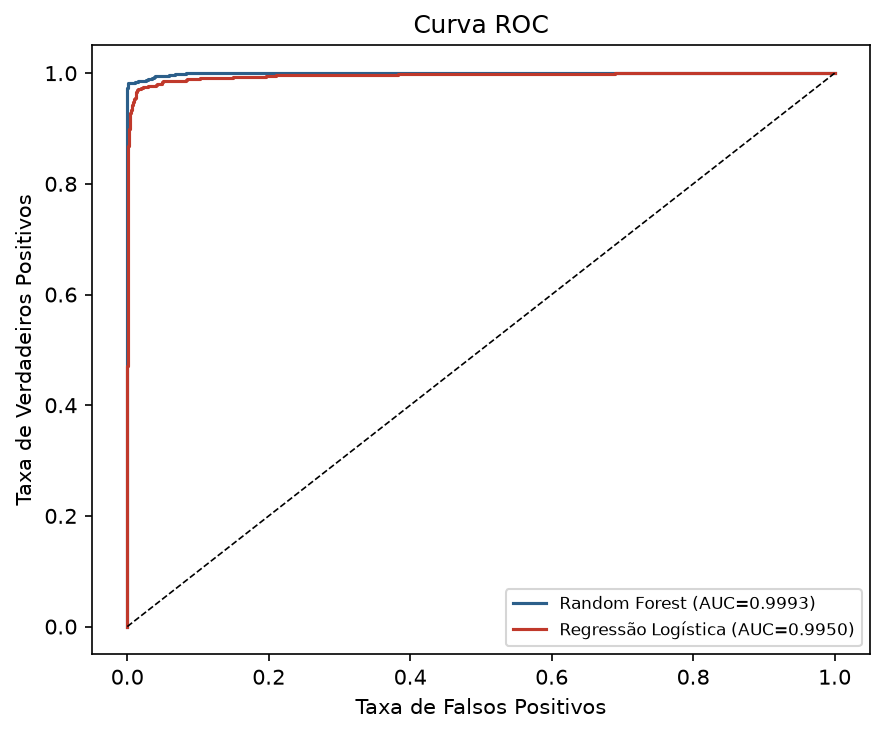
\includegraphics[width=0.48\textwidth]{fig6_roc_curve.png}
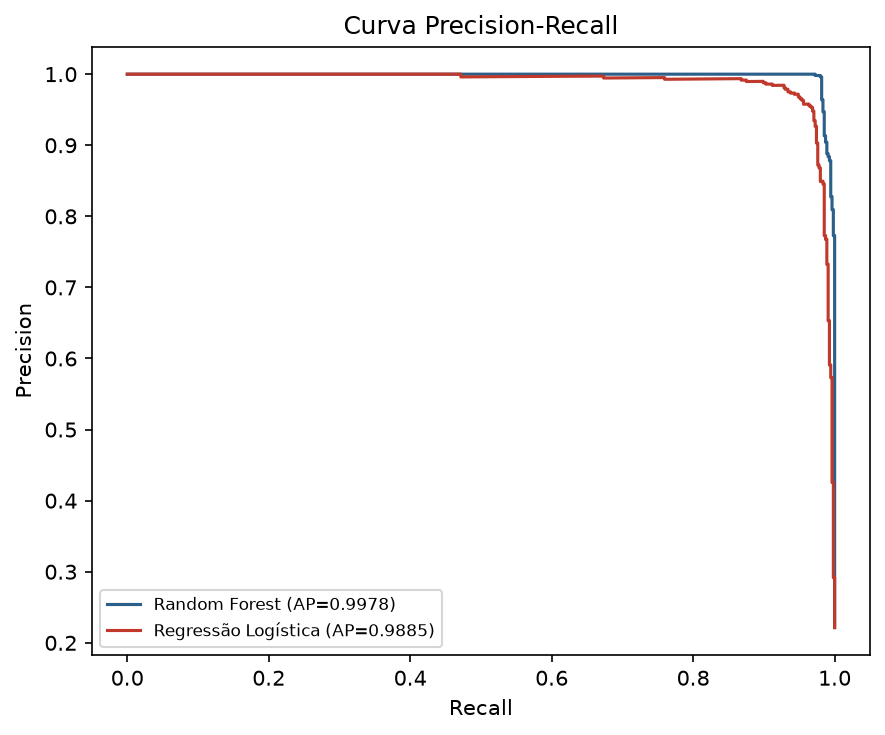
\includegraphics[width=0.48\textwidth]{fig7_pr_curve.png}
\caption{Curvas ROC (esquerda) e Precision-Recall (direita) dos
modelos otimizados.}
\label{fig:curves}
\end{figure}

\subsection{Interpretação dos Atributos}

A análise dos atributos mais relevantes permite compreender quais
características do comportamento transacional mais contribuem para a
identificação de fraude. A Figura \ref{fig:rf} apresenta a importância
dos atributos segundo o Random Forest, e a Figura \ref{fig:lr} os
coeficientes da Regressão Logística.

\begin{figure}[H]
\centering
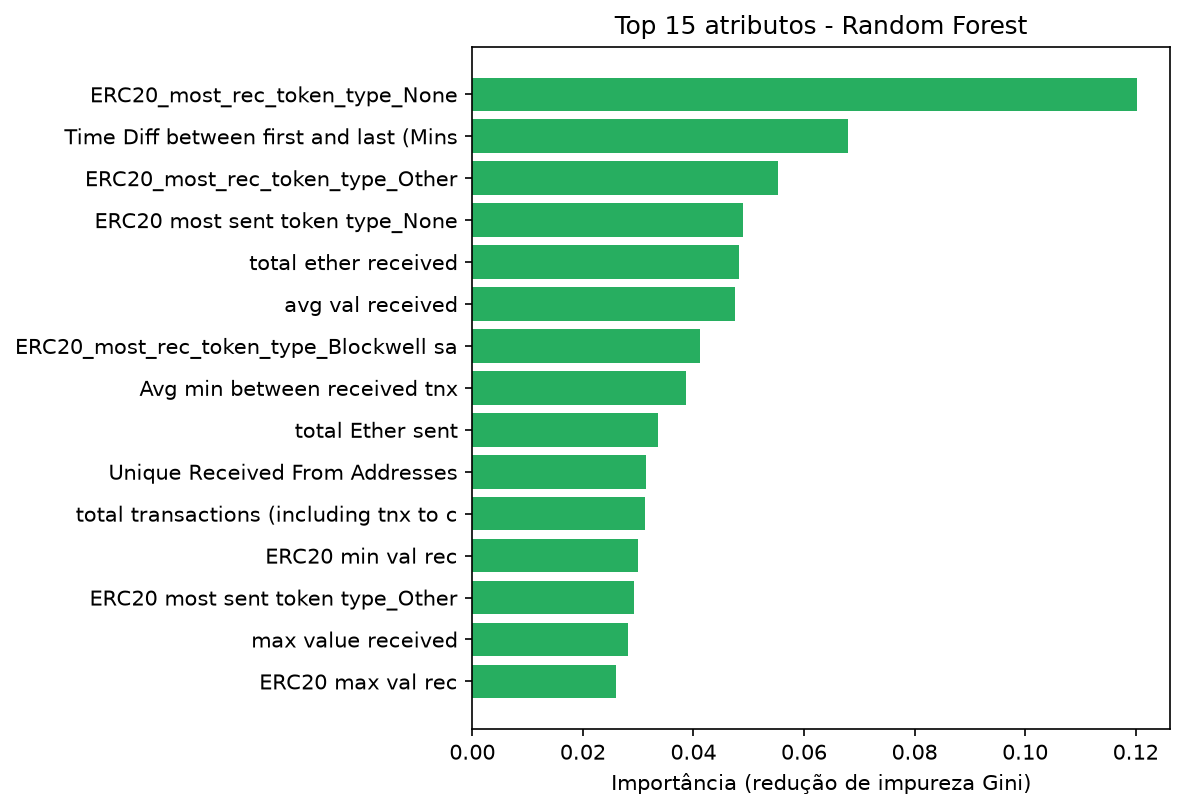
\includegraphics[width=0.8\textwidth]{fig4_rf_importances.png}
\caption{Atributos mais importantes segundo o Random Forest.}
\label{fig:rf}
\end{figure}

\begin{figure}[H]
\centering
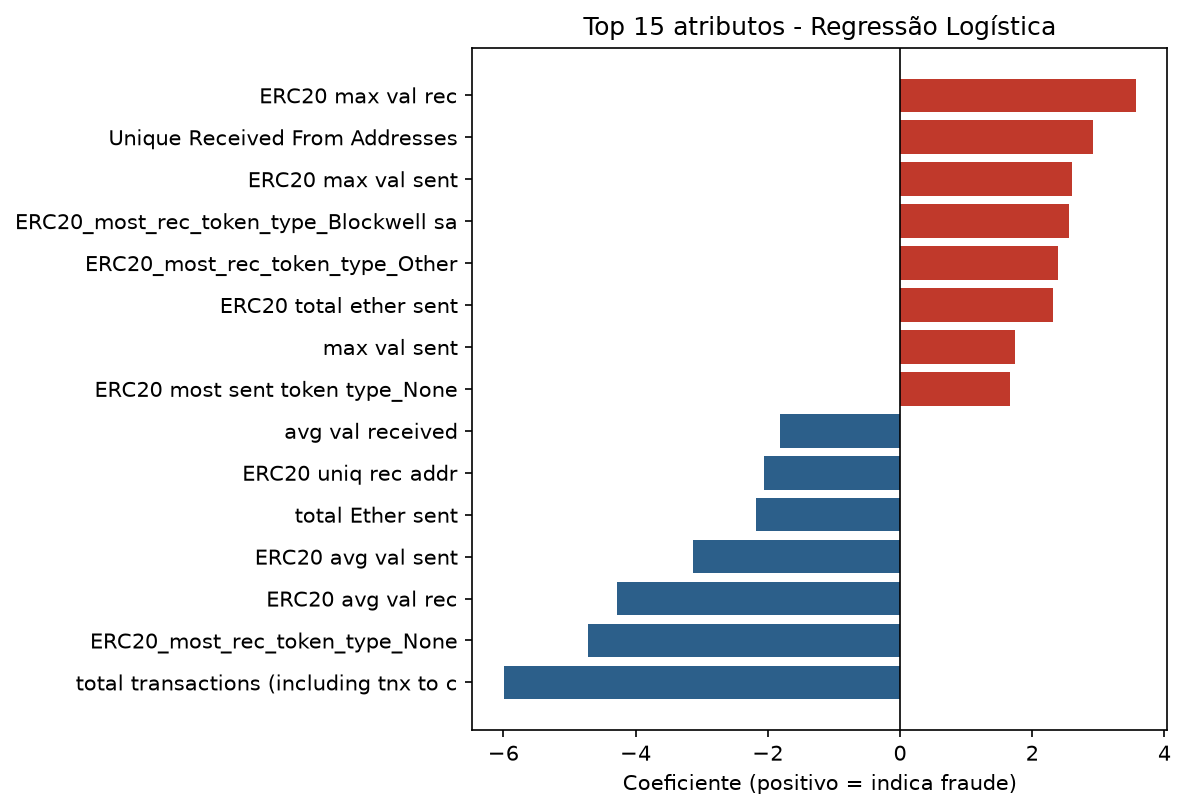
\includegraphics[width=0.8\textwidth]{fig5_lr_coefficients.png}
\caption{Atributos de maior peso na Regressão Logística (coeficientes
positivos indicam fraude).}
\label{fig:lr}
\end{figure}

Os dois modelos convergem para padrões interpretáveis e consistentes.
A ausência de recebimento de tokens ERC20 destacou-se como o atributo
mais importante no Random Forest, sugerindo que contas fraudulentas
tendem a apresentar atividade transacional mais restrita, limitada à
movimentação de Ether. Na Regressão Logística, o número total de
transações apresentou o coeficiente negativo de maior magnitude,
indicando que contas com histórico transacional extenso tendem a ser
legítimas; em contrapartida, contas fraudulentas frequentemente se
comportam como ``carteiras de passagem'', utilizadas em poucas
operações antes de serem abandonadas -- padrão característico de golpes.

\subsection{Limitações}

Algumas limitações devem ser consideradas. O \textit{dataset} descreve
o comportamento das contas de forma agregada, não contemplando a
sequência temporal das transações, o que poderia revelar padrões
dinâmicos de fraude. Além disso, os rótulos refletem fraudes já
identificadas, podendo não capturar modalidades emergentes de golpe.
Por fim, o desempenho elevado dos modelos, embora positivo, sugere a
necessidade de validação em dados mais recentes e diversos para
confirmar a capacidade de generalização.

\section{Conclusões e Trabalhos Futuros}

Este trabalho aplicou o processo de mineração de dados CRISP-DM à
detecção de contas fraudulentas na rede Ethereum, comparando seis
algoritmos de classificação. O Random Forest destacou-se como o modelo
mais eficaz, atingindo F1-score de 0,9832 e AUC-ROC de 0,9993 no
conjunto de teste, sem nenhum falso positivo, atendendo ao objetivo de
mineração proposto.

Entre as lições aprendidas, destaca-se a importância do diagnóstico
cuidadoso da qualidade dos dados -- como a identificação de
representações inconsistentes de valores ausentes e de colunas
redundantes -- e a confirmação prática de que o algoritmo \textit{Naive
Bayes} é inadequado para conjuntos com atributos correlacionados e de
tipos mistos. A interpretação dos atributos mostrou-se tão valiosa
quanto o desempenho preditivo, ao revelar padrões comportamentais
associados à fraude.

Como trabalhos futuros, sugere-se a incorporação de atributos
temporais e de grafo (relações entre endereços), a exploração de
técnicas de \textit{ensemble} adicionais e a avaliação dos modelos em
conjuntos de dados mais recentes, a fim de verificar sua robustez
frente à evolução das estratégias de fraude.

\begin{thebibliography}{}

\bibitem{fayyad1996}
Fayyad, U., Piatetsky-Shapiro, G. and Smyth, P. (1996) ``Knowledge
discovery and data mining: towards a unifying framework'', In:
Proceedings of the Second International Conference on Knowledge
Discovery and Data Mining (KDD'96), AAAI Press, p. 82--88.

\bibitem{tan2009}
Tan, P.-N., Steinbach, M. and Kumar, V. (2009) ``Introdução ao Data
Mining: Mineração de Dados'', Editora Ciência Moderna, Rio de Janeiro,
1ª edição.

\end{thebibliography}

\end{document}
